\section{Evaluation}
\label{sec:eval}

We evaluate RCuckoo by directly comparing its performance in terms of
latency and throughput with other state-of-the-art disaggregated key
value stores. We substantiate our design decisions through a series of
micro-benchmarks. Specifically, we measure throughput as a function of
hashing locality, covering read threshold, and choice of search
algorithm.

\section{Implementation}

Our implementation of RCukcoo consists of a of 8.7k C++
implementation and a 12k line Python implementation which
simulates RDMA. Both implementations will be made available
on Github.  All results reported in Section~\ref{sec:eval}
are from the C++ implementation. At the time of writing only
the python implementation includes support for delete
operations, and extent entries. As such all C++ results are
for inserts, reads, updates and inlined table operations.
RCuckoo is designed for ConnectX-5 NICs. It uses OFED-4.9
which supports experimental verbs for atomic masked CAS and
device mapped memory. 


\begin{figure*}[ht]
    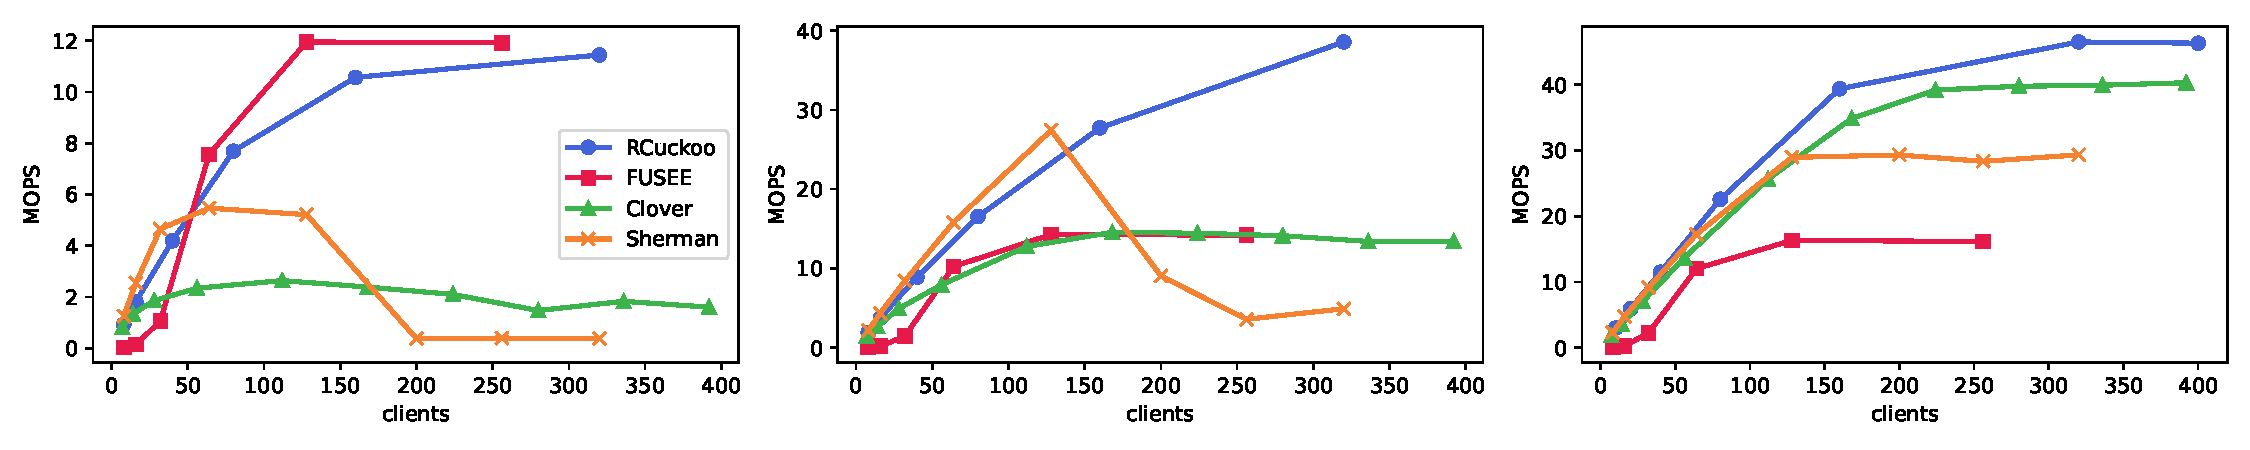
\includegraphics[width=0.99\linewidth]{fig/hero_ycsb_throughput.pdf}

    \caption{Throughput as a function of the number of clients for three different workloads (Zipf $\theta$=0.99): \textbf{(a)} YCSB-A 50\%
    read 50\% update, \textbf{(b)} YCSB-B 95\% read 5\% update and \textbf{(c)}
    YCSB-C 100\% read.}
    \label{fig:ycsb_throughput}
 \end{figure*}


\subsection{Testbed}

We conduct our evaluation on an 11-node cluster of dual-socket Intel
machines. Each CPU is an Intel Xeon(R) E5-2650 clocked at
2.20~GHz. Each machine has 256~GB of RAM with 128~GB per NUMA
node. All machines have a single dual-socket ConnectX-5 attached to a
100-Gbps Mellanox Onyx switch. In our RCuckoo experiments we use one
sever as the memory server and the rest a client machines
spreading threads evenly across machines.

%\subsection{Comparision systems}

We compare RCuckoo against three recent RDMA key-value stores with
different designs.  While none have the same assumptions or feature
set as RCuckoo, each represents an apt comparison point for different
aspects.

We directly compare RCuckoo against three disaggregated
key-value stores Fusee~\cite{fusee}, Clover~\cite{clover},
and Sherman~\cite{sherman}. Each system has distinct design
tradeoffs. 
%%
Fusee is the nearest system to RCuckoo in our design space.
It is fully disaggregated and uses optimistic inserts rather
than locks. Fusee is based on race hashing which uses 64 bit
width index entries set with CAS to point to extent entries.
Fusee is the closest comparison we have to illustrate the
tradeoffs between locks and optimistic concurrency.
%%
Clover is a partially disaggregated system which uses
two-sided RDMA operations to modify the index and one-sided
operations for updates, deletes, and reads.
%%
Sherman a disaggregated B-Tree and the only system at the
time of writing which uses locks and not optimistic
concurrency to guard its index. Our performance comparison
with Sherman is not apples to apples. Sherman maintains
ordered key-value pairs for range queries and thus has
higher overheads on updates than the other systems.

\textbf{FUSEE}
is a key-value store designed for full
disaggregation~\cite{fusee}.  It is built on top of RACE~\cite{race}
with extensions to support replication in the face of contention.
While RACE represents a more direct comparison to RCuckoo, no open
source implementation of RACE is available.  Instead, we deploy FUSEE
with a single memory node to effectively remove the overhead of
replication.  FUSEE/RACE hashing uses fixed-sized 64-bit index entries
to in order to employ RDMA compare-and-swap operations for updates. As
such, RACE-based systems cannot store key-value pairs in the index
table itself and require a second round trip even for reads of small values.
%on reads to recover
%extent entries which contain full key value pairs.

\textbf{Clover}
is a key-value store designed for remote persistent memory~\cite{clover}. It
does not support full disaggregation; instead, its index structure is
managed by CPU cores on a metadata server. However, its
persistent-memory updates are implemented using one-sided RDMA
operations.  Moreover, unlike FUSEE---and similar to RCuckoo---Clover
reads are self verifying.
%Clover uses index caching to optimize reads.  When re-reading key-value
%entires clover can as it directly
%reads the entry without negotiating with the index.
In contrast to prior Clover comparisons~\cite{fusee} that force
clients to read from the server's index on each read, we allow Clover
to take advantage of its client caching algorithm to achieve near
RDMA line-rate performance.

\textbf{Sherman}
is a B-tree designed for remote memory~\cite{sherman}.
%and high write
%throughput.
Unlike Clover and FUSEE which employ optimistic consistency control,
Sherman uses locks to guard updates similar to RCuckoo.  On the other
hand, Sherman clusters are not fully disaggregated: each node in a
cluster is a peer with many CPU cores and a single memory core
that is responsible for servicing allocation RPC calls from clients.
%Unlike the other systems
%Sherman is cluster based, and does not support a having
%isolated memory machines.
%All machines are equal nodes in a
%cluster and run both a memory controller and client threads.
As such, Sherman does not encounter the same bandwidth bottlenecks as
the other systems because requests are partitioned across all
machines in the cluster.
%However, it assumes that colocated clients can resolve lock
%contention locally and clients colocated with their segment
%of the B-Tree can perform local operations. These
%assumptions enable sherman to have high performance under
%contention even though it uses locks and manages a more
%complex data structure than the unordered key-value stores.
%While Sherman does not meet the fully disaggregated model it
%does provide a good comparison for RCuckoo as it is the only
%other system to use locks in remote memory.


% \subsubsection{Clover}
% \todo{insert a short clover description}

\begin{figure*}[ht]
    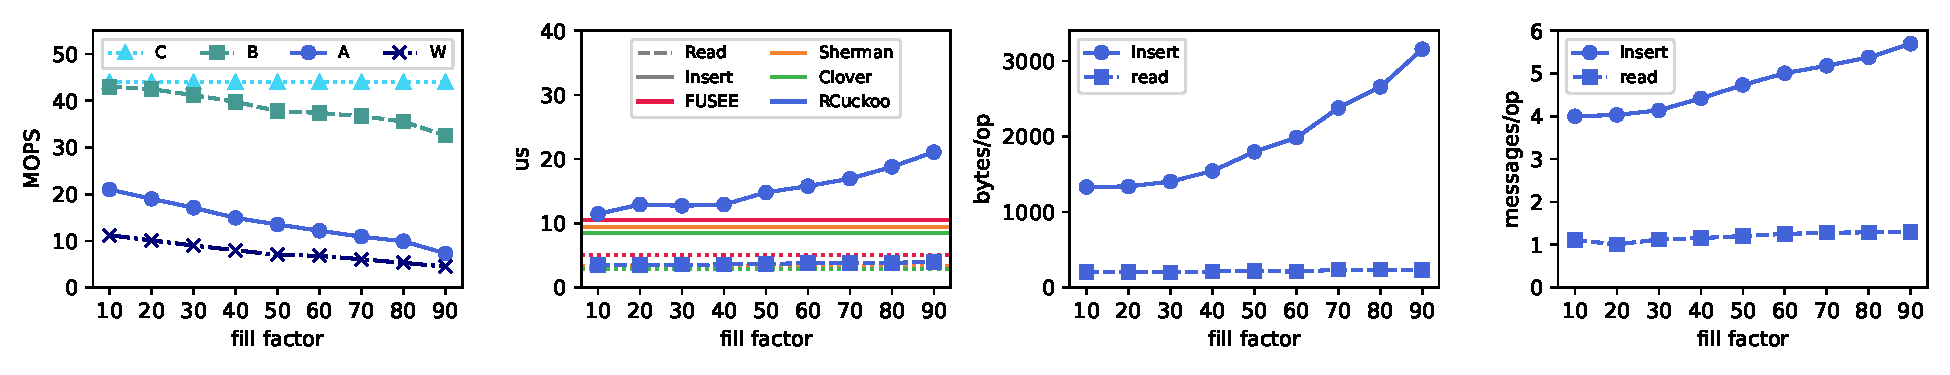
\includegraphics[width=0.99\linewidth]{fig/hero_ycsb_fill.pdf}

    \caption{Insert and read performance as a
    function of fill factor. \textbf{(a)} Throughput for four different workloads. \textbf{(b)}
    Median operation latency, \textbf{(c)} average operation size, and \textbf{(d)}
    average messages per operation under YCSB-A.}

    \label{fig:ycsb_fill}
\end{figure*}

% \begin{figure}[ht]
%     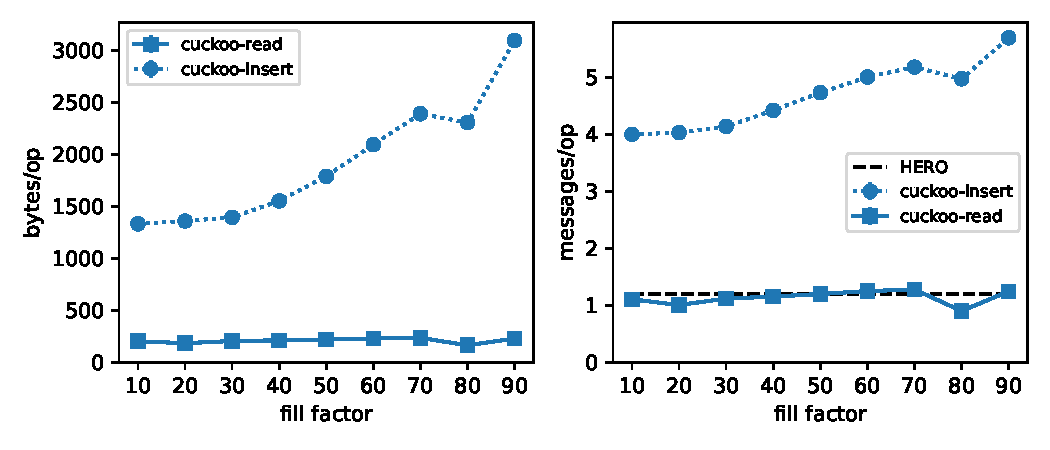
\includegraphics[width=0.99\linewidth]{fig/hero_ycsb_fill_ops_bw.pdf}
%     \caption{YCSB-A workload messages and bandwidth per operation as a function of fill factor}
%     \label{fig:ycsb_fill_ops_bw}
% \end{figure}



\subsection{Performance}

We start by considering the classical YCSB workloads which employ
varying mixes of read and update operations before turning to the
more complex insert operation.

\textbf{YCSB:}
Figure~\ref{fig:ycsb_throughput} shows the throughput in terms of
operations per section of RCuckoo, FUSEE, Sherman, and Clover for
three different YCSB workloads with a Zipf(0.99) distribution. YCSB-A
is a 50\% read 50\% update, YCSB-B is 95\% read and 5\% update, and
YCSB-C is 100\% read.  In each experiment a variable number of clients
insert 90-M entries containing 32-bit keys and 32-bit values into a
100-M-entry hash table.


On YCSB-A RCuckoo tops out after approximately 160 clients due to lock
contention on hot keys.  FUSEE's maximum performance is slightly lower
due to its requirement for an additional round trip per operation (to
retrieve the extent). Sherman keeps pace until about 5 MOPS at which
point it suffers from lock contention due to its B-Tree structure.
(Sherman and RCuckoo perform similarly for uniform workloads where
lock contention is less of an issue.).  Clover performs the worst
under write-heavy workloads due to the inability to effective leverage
client-side caching of its constantly changing index structure.

On read mostly and read-only workloads (YCSB-B and C)
RCuckoo extracts even further benefit over FUSEE from its ability to
complete read in a single round trip rather than two and gains
additional benefit by collapsing most reads into a single packet
(Section~\ref{sec:read_threshold}).  Sherman performs well on
read-mostly workloads as it can directly read from the B-Tree in a
single round trip without the need for pointer chasing, but it
continues to bottleneck on lock contention in YCSB-B due to hot
keys. While Sherman experiences no such bottleneck on YCSB-C its read
algorithm is more complex than RCuckoo's leading to lower top-end
performance. Clover performs similarly to FUSEE on YCSB-B, and is the
most competitive with RCuckoo in read-only sceario.  When it is able
to leverge its client index cache, Clover's reads are very similar to
RCuckoo in that they require only a single 1-sided RDMA read;  we
suspect that with tuning Clover's read-only performance
could be brought to par with RCuckoo.

\textbf{Inserts:}
%%
%By default YCSB-A,B,C use updates. RCuckoo's insert
%algorithm is it's most complex and bandwidth intensive
%component. In this section

RCuckoo insert operation is high performance despite
containing nearly all of our algorithms complexity. Inserts
are more expensive when cuckoo indexes are nearly full so we
report insert performance as a function of the indexes fill
factor. To show how RCuckoo responds to insert heavy
workloads we modify YCSB to perform \textbf{inserts rather
than updates}. All experiments in Figure~\ref{fig:ycsb_fill}
use inserts rather than updates, for example YCSB-A is 50\%
update and 50\% read. YCSB-W is a write only or 100\% insert
workload.
%%
Figure~\ref{fig:ycsb_fill}(a) shows the aggregate throughput
of 400 clients across four different workloads as a function
of the table's fill factor.  As the index table fills,
cuckoo paths become longer leading to increased contention
and additional bandwidth consumption from larger covering
reads. In each case (except YCSB-C) RCuckoo's performance
declines with fill factor. In the insert-only YCSB-W case
RCuckoo's performance drops from 11.5 to 4.5 MOPS.  As a
point of comparison, FUSEE's maximum insert-only performance
is 9.1 MOPS on our testbed, although it is independent of
fill factor.  While FUSEE out-performs RCuckoo at high fill
factors, we observe that an insert-only workload is uncommon
in practice~\cite{facebook-memcached}.

We plot operation latency, size, and message counts (in
terms of RDMA packets) as a function of fill factor in
Figure~\ref{fig:ycsb_fill}(b--d).  For comparison, we report
latency values of insert and read operations for the
comparison systems. These values were not collected under
load and represent best-case performance on our testbed.
Read latency is nearly identical for all systems save FUSEE,
as it requires an additional round trip.  Insert times vary:
Clover and Sherman use two-sided RDMA operations for insert
and both need to perform allocations and set up metadata for
the requesting client.  FUSEE is slightly slower, roughly
the same as RCuckoo's best-case.  As the table fills,
however, cuckoo paths grow in length causing RCuckoo insert
operations to require additional round trips to find valid
cuckoo paths.  At maximum fell, insert operations take
roughly twice as long as in an empty table. This rising cost
is reflected by the increase in both bytes and messages per
operation.  RCuckoo reads, on the other hand, have roughly
the same cost and performance regardless of fill factor.


\begin{figure}[t]
    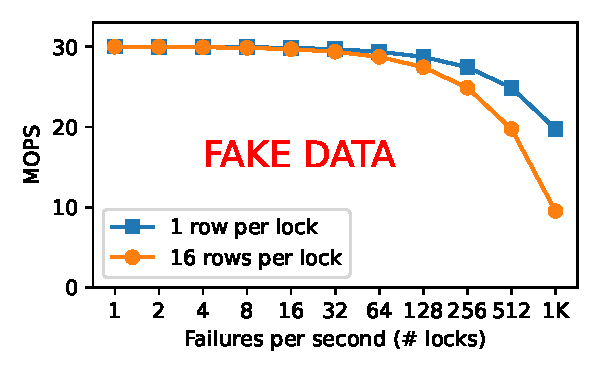
\includegraphics[width=0.99\linewidth]{fig/failure_throughput.pdf}
    \caption{Throughput vs failure rate.}
    \label{fig:failure_throughput}
    \vskip -1em
\end{figure}

\subsection{Fault tolerance}

RCuckoo runs at nearly full throughput during realistic
failure scenarios and remains functional in the face of
hundreds of failures per second. When a client fails while
holding a lock the lock is stranded and requests for that
lock will block until after a client times out and reclaims
the lock.
%%
We emulate hundreds of client failures per second by
performing a partial insert operation which truncates the
batch of insert packets including lock releases. The table
entries are left in one of the inconsistent states listed in
Section~\ref{sec:table-repair} and locks are left set.


Figure~\ref{fig:failure_throughput} illustrates RCuckoos
ability to operate at high throughput in the face of
failures. Lock granularity increases the probability that
multiple clients will block on the same failed lock. Larger
locks have little difference when failures are semi-frequent
and have a larger impact as hundred of failures occur per
second.  The performance impact of a few number of failures
per second is low which is ideal considering that failures
in RDMA clusters are relatively rare.  As a point of
reference, we observe that RCuckoo can still operate despite
thousands of failures per second while a server can only
establish approximately 1.4~K RDMA connections per second
using state of the art techniques~\cite{xrdma}.

\subsection{Dependent hashing and search}

\begin{figure}[ht]
    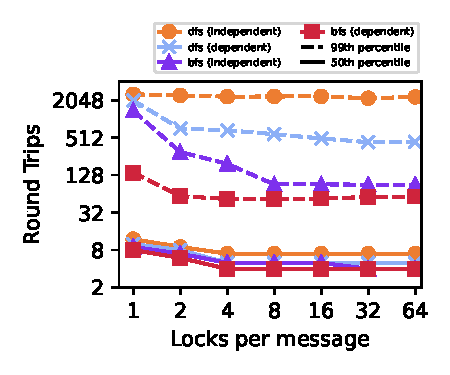
\includegraphics[width=0.99\linewidth]{fig/search_dependence.pdf}

    \caption{ Search function performance with independent
    and dependent hashing.}

    \label{fig:search_dependence}
\end{figure}

Hash dependence and search function choice have the highest
impact on RCuckoo's performance. Dependent hashing reduces
the probability locks are scattered throughout the table
which enables RCuckoo to combine lock requests into a few
masked CAS messages. Simultaneously search function choice
dramatically affects the length of cuckoo paths. BFS
produces much shorter paths than
DFS~\cite{cuckoo-improvements,pilaf,cuckoo}.
Figure~\ref{fig:search_dependence} illustrates the effect of
search function and dependent hashing on RCuckoo's inserts.
We vary the number of locks per message to demonstrate the
effect of path length and show why masked cas plays an
important role in RCuckoo's performance. We measured both
the median, and 99th percentile round trips per request on a
table with 100M entries. We fille the table to 85\% and then
executed insert operations to 95\%.

DFS with no hash dependence has extremely poor performance
at it's tail, taking over 2K round trips to complete. Both
at it's median and 99th percentile it sees only small
benefits from setting multiple locks per request as the
locks are scattered throughout the table. DFS with
dependence has far lower tail latency, and improves the
number of locks which can be acquired per message, however
it still constructs long rather than minimum length paths.
BFS with dependence provides the best performance and gains
the most from setting more locks per request. At 64 locks
per request it has 7.5x lower round trips at it's 99th
percentile and 4 rather than 5 round trips on average. We
found that A* search provided the same minimal path length
as DFS with slightly better locality. It's performance
against BFS was only superior at fill factors above 95\% and
lower elsewhere due to a higher runtime cost on short paths.



% Hash function locality hash a major impact in rcuckoo's
% performance.  Acquiring locks can only be done in a few
% round trips when the locks are clustered together tightly in
% the lock table.  Furthermore, the search function used to
% determine the cuckoo path has a large impact on the locality
% of the locks necessary to lock the path. We evaluate
% dependent hashing and independent hashing as well as random
% and a* search. We measure the number of round trips required
% for each control as a function of the number of locks which
% can be acquired per round trip.

% Figure~\ref{fig:search_dependence} shows the performance
% improvements gained by both locality hashing and A* search.
% In this experiment the table is filled from 0 to 90\% full
% with a ycsb-w workload. We measure the 99th percentile of
% round trips for these workloads. Random search with
% independent hashing leads to a large number of round trips
% as locks are scattered throughout the table. RDMA masked CAS
% operation do little here to reduce the round trips as they
% can rarely aquire more than one lock in a round trip. With
% dependent hashing and random search RDMA CAS operation are
% almost sufficient to reduce round trips, however the absolute
% number of locks required per insert is high which leads to
% greater contention. A* search with dependent hashing has
% cuckoo paths that are both short, and clustered together.


\begin{figure*}[t]
    \centering
    \begin{subfigure}{0.3\linewidth}
        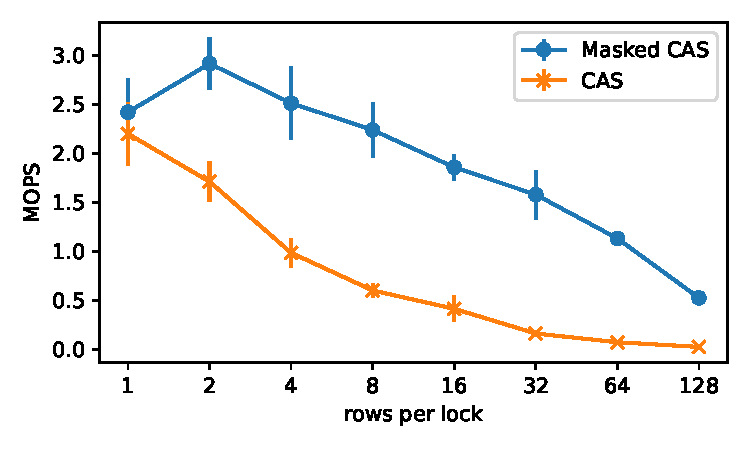
\includegraphics[width=0.99\linewidth]{fig/masked_cas_lock_size.pdf}
    \end{subfigure}
    \begin{subfigure}{0.3\linewidth}
        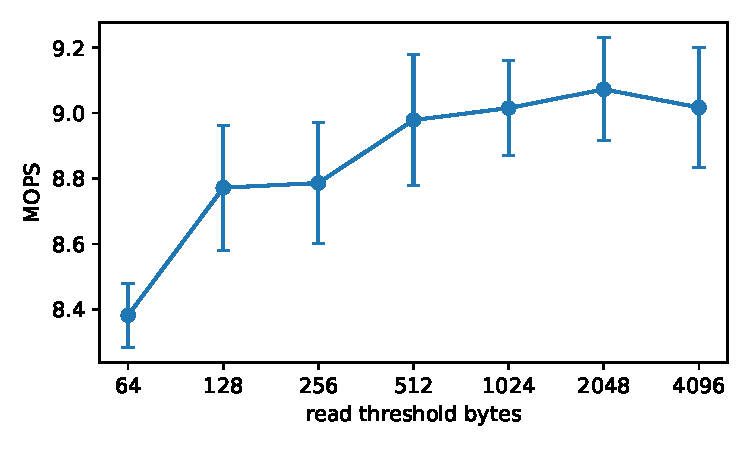
\includegraphics[width=0.99\linewidth]{fig/read_size.pdf}
        % \label{fig:hash_factor}
        % \caption{}
    \end{subfigure}
    \begin{subfigure}{0.3\linewidth}
        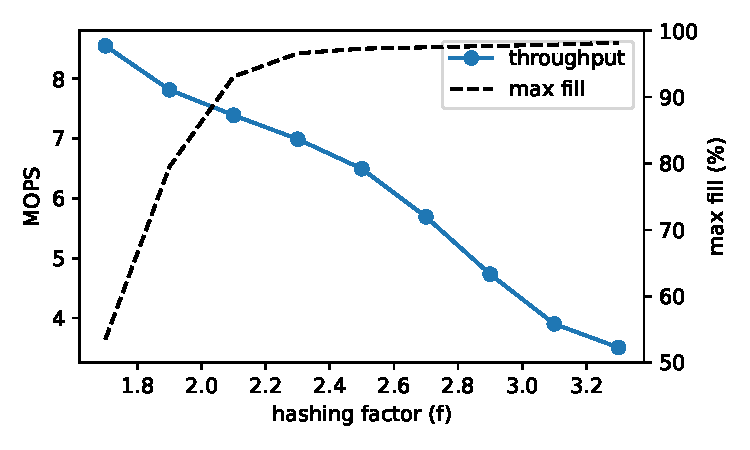
\includegraphics[width=0.99\linewidth]{fig/factor.pdf}
        % \label{fig:hash_fill}
        % \caption{}
    \end{subfigure}.
    \vspace{-1em}
    \caption{
    \textbf{(a)} Masked CAS vs Unmasked CAS throughput.
    \textbf{(b)} Read threshold vs throughput.
    \textbf{(c)} Exponential factor relation to max fill in cuckoo hash.
    }
    \label{fig:performance_breakdown}

\end{figure*}

\subsubsection{Masked CAS}

Under contention masked CAS operations provide a significant
performance improvement. We measure it's benefit in terms of
throughput by comparing it with default CAS. In the
default case, when acquiring locks clients set the lock bits
for the locks they require and set all other bits in the cas
to 0. If the cas fails the current state of the lock table
over that range is returned as a result to the client and
the client tries to aquire their locks again using the
updated state of the lock table. Masked compare and swaps
are issued with the minimal mask required to set the locks.

Figure~\ref{fig:performance_breakdown} shows the improvement
gained by masked CAS. Default CAS operations perform better
with fewer rows per lock, as the probability of a lock being
set within the 64bit range is at its lowest. At higher rows
per lock CAS suffers from failed lock acquisitions from both
contested locks and due to a lack of synchronization. In
contrast masked CAS sees an improvement when two rows per
lock are used, as more second search attempts succeed, and
only suffers from direct lock contention as the rows per
lock increase.


\subsection{Hash Function Factor $f$}

Low hash factors $f$ have higher performance due to better
locality at the tradeoff of their maximum fill factor. The
relationship between $f$ and performance is nearly linear,
while the relationship between $f$ and fill factor is
exponential. Figure~\ref{fig:performance_breakdown}(c) shows
the relationship between $f$, the max fill rate, and insert
performance. These numbers were collected on an insert only
workload with 100 million table entries. We choose an $f$ of
2.3 in practice as it has the highest product of fill factor
and throughput.

\subsection{Read Threshold Performance}
\label{sec:read_threshold}
As described in section ~\ref{sec:reading} rcuckoo uses a
read threshold to capture both hash locations if the
locations are within a defined read threshold.
Figure~\ref{fig:performance_breakdown}(b) shows the
performance gains from increasing the read threshold. Here
each row is 64 bytes so our minimum threshold of 64 ensures
two packets are issued for each read request. We limit the
number of clients to 40 so that their is plenty of bandwidth
to support the inflated reads. Higher read thresholds trade
off network bandwidth for operation latency. When bandwidth
is plentiful large windows can improve throughput but up to
8\%.

% \begin{figure}[ht]
%     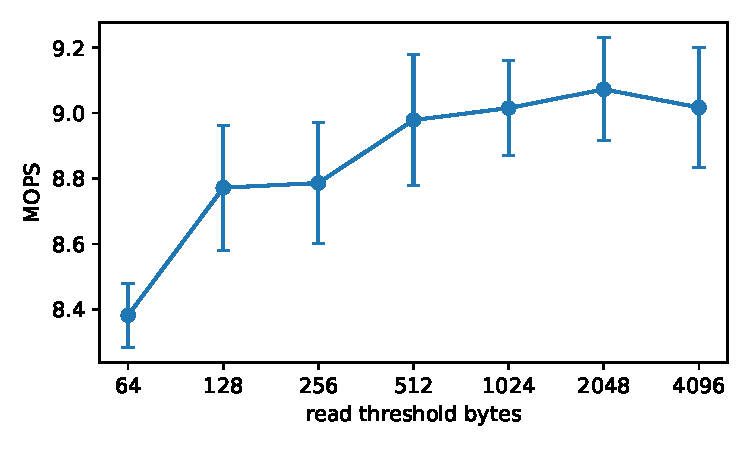
\includegraphics[width=0.99\linewidth]{fig/read_size.pdf}
%     \caption{Read Threshold vs Throughput}
%     \label{fig:read_threshold}
% \end{figure}


\subsection{Entry Size}
\begin{figure}[ht]
    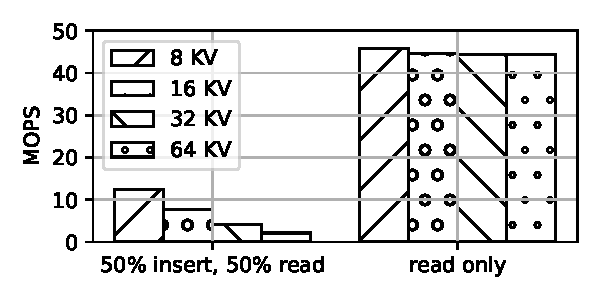
\includegraphics[width=0.99\linewidth]{fig/entry_size.pdf}
    \caption{Throughput vs KV entry size}
    \label{fig:entry_size}
\end{figure}

Key value pairs embedded directly in the index enable single
round trip reads, at the cost of inflating the bandwidth of
operations. We run a 50\% read 50\% insert and a read only
workload to illustrate the overhead of larger entries.
Figure~\ref{fig:entry_size} shows the effect of key value
pair size on operation throughput. Insert quickly saturates
the network bandwidth. At 16 byte KV entries the network
bandwidth is fully absorbed at 8MOPS. Reads which have lower
bandwidth requirements see very little chance in throughput
across entry sizes. We suggest that known read heavy
workloads should use inlined entries as reads see a large
boost in performance. Update operations are similarly
unaffected by entry size up to 64 bytes. 

% Our design choice
% in embedding KV pairs is motivated by networking trends
% which suggest that 800 GBPS and higher network speeds will
% be available in the coming years. While round trip latency
% is expected to remain largely the same.

\subsection{Search Success}
\label{sec:search_success}
\begin{figure}[ht]
    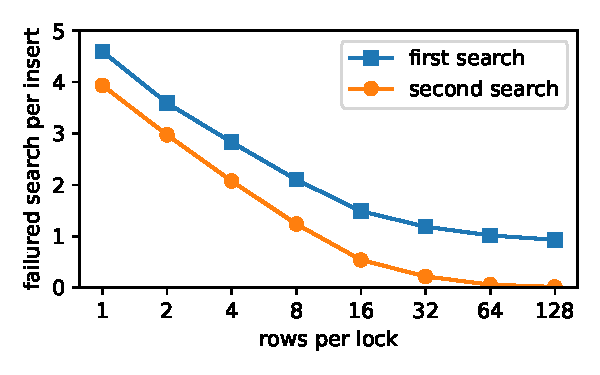
\includegraphics[width=0.99\linewidth]{fig/search_success_lock_size.pdf}
    \caption{Failure rate of search algorithms vs lock size under high contention}
    \label{fig:search_success}
\end{figure}

RCuckoo's two stage search algorithm is designed to improve
the probability that an insert will be successful given that
a clients local cache is out of sync. To demonstrate the
effectiveness of our two stage search strategy we measure
the success rate of our searches under high contention. With
400 concurrent clients we fill a small table (10M entries)
up to 85\% prior to measuring success rate in order to
maximize cuckoo path length. Figure~\ref{fig:search_success}
shows the failure rate of both search stages. The first
search is the success rate of a search based entirely on
cached information. The second search is the success rate of
our restricted search performed after acquiring locks. We
measure the response of both as a function of lock size.
Given 1 row per lock the failure rate of both searches is
over 4 as the local cache is almost always out of sync, and
retries are not guaranteed to be synchronized. As lock
granularity grows the frequency of second search success
drops dramatically. At 64 rows per lock our second search
succeeds 95\% of the time even when the cached search fails
at a rate of 99\% per insert.



